\section{Introduction}
\label{sec:introduction}

Large language models act in the world through \emph{agents}: a model embedded
in a harness---the software that supplies its system prompt, tools, skills,
context policy, and control loop~\citep{weng2026harness,anthropicagents,react,
toolformer,sweagent,autogen,voyager,webarena,osworld}.  How much of a model's
capability becomes measurable progress is decided by that harness, nowhere more
sharply than in \emph{discovery}, where a frozen LLM paired with a hand-built
evolutionary scaffold produces mathematical and algorithmic results beyond
strong baselines~\citep{funsearch,alphaevolve,alphaevolvemath,openevolve,
shinkaevolve,eoh,llmsr,aiscientist}.  A natural next step is
\emph{self-improvement}: letting an agent get better at a task from its own
experience, with no stronger model to learn from.  Today this takes one of two
forms (Figure~\ref{fig:taxonomy}a,b).  One updates the model's \emph{weights},
fine-tuning the executor on its own rollouts, as in test-time and reasoning
RL~\citep{tttdiscover,thetaevolve,ttrl,ttt,grpo,dapo,agenticrl,ragen}.  The
other keeps the model frozen and edits its \emph{harness}---prompts, tools,
context, or an external program archive---as an artifact revised by a
\emph{fixed} proposer~\citep{openevolve,funsearch,shinkaevolve,eoh,metaharness,
selfharness,hase,dgm,sica,godelagent,stop,alita,selfevolvesurvey}.

\begin{figure*}[t]
\centering
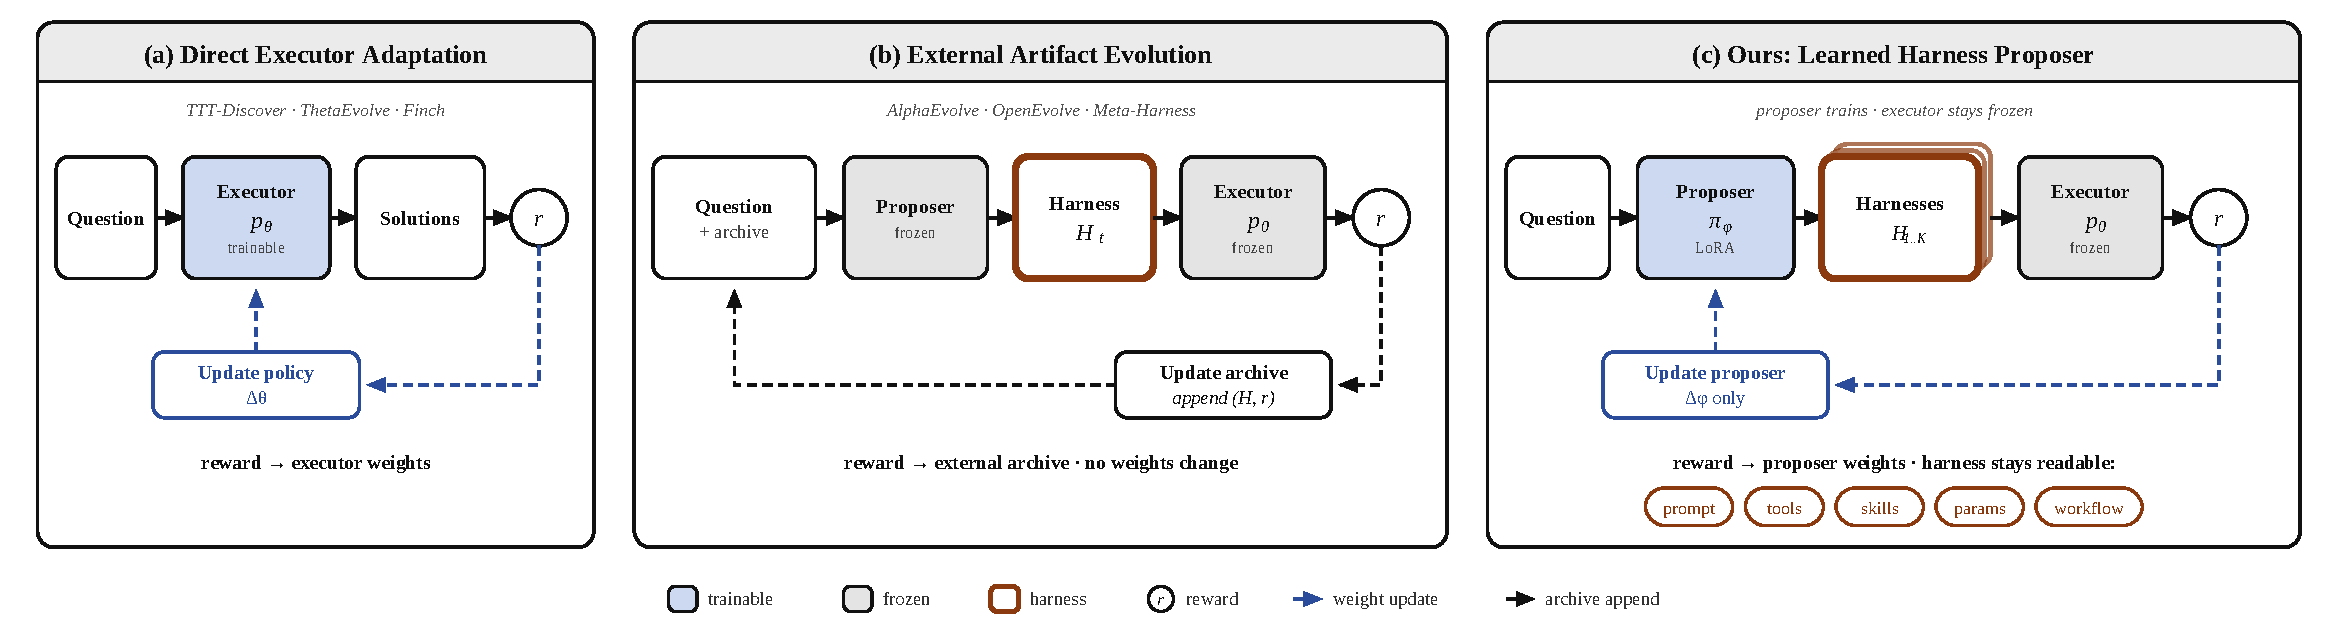
\includegraphics[width=\textwidth]{figures/harness_taxonomy.pdf}
\caption{\textbf{Where does the reward go?}  Three ways to improve an agent from
its own experience.  \textbf{(a)}~\emph{Direct executor adaptation}
(TTT-Discover, ThetaEvolve, Finch): the reward updates the executor's own
weights, so the policy that solves the task is also the policy that is trained.
\textbf{(b)}~\emph{External artifact evolution} (AlphaEvolve, OpenEvolve,
Meta-Harness): the executor stays frozen and the reward is appended to an
external archive or harness, which a \emph{fixed} proposer reads back.
\textbf{(c)}~\emph{\method{} (ours)}: a trainable proposer emits harnesses
$H_{1:K}$---prompt, tool descriptions, skills, and control parameters---for a permanently
frozen executor, and only the proposer is updated.  Adaptation is thus separated
from execution and routed through an explicit, inspectable artifact.}
\label{fig:taxonomy}
\end{figure*}

Both routes stop short of a reusable \emph{proposer}, in complementary ways.
Weight updates train on hundreds of rollouts per
step~\citep{tttdiscover,thetaevolve}, register their gains only as diffuse
weight changes---never as a nameable tool, skill, or procedure---and are
unavailable when the executor is frozen by policy, safety review, or an API
boundary.  Harness editing keeps its \emph{proposer} fixed: the same
prompt-optimizer, textual-gradient, or agent-design
procedure~\citep{ape,opro,promptbreeder,evoprompt,mipro,metaprompting,dspy,
textgrad,trace,gepa,adas,aflow,agentsquare,agentsymbolic} re-derives design
knowledge from scratch on every run, with nothing amortized into the
proposer itself.  History suggests the resolution: hand-designed pipelines
gave way to searched ones, and searched ones to \emph{learned}
components~\citep{learn2learn,hypernetworks,adas}.

We propose to learn the proposer itself (Figure~\ref{fig:taxonomy}c).
\method{} keeps the executor $M_0$ \textbf{permanently frozen} and trains a
harness \emph{proposer} $\pi_\phi$ by group-relative RL adapted for
discovery (\S\ref{sec:method}) to emit, per task, a complete harness:
system prompt, skill playbook, tool descriptions, control parameters, and,
through a generative channel, \emph{new executable tools} as Python
source~\citep{latm,creator,craft,voyager,trove}.  Each spec compiles
deterministically into a runnable agent; the frozen executor rolls it out
under a hard evaluator budget; and a group's relative outcomes are the
proposer's only task-level signal (Figure~\ref{fig:overview}).  Round over
round, the proposer internalizes the task's reward history into its weights
rather than into an ever-growing context.

Three properties motivate this design.  \emph{Amortization}: search cost
is paid at training time, so a new round costs a handful of proposer
episodes rather than a fresh scaffold search---the argument behind learned
optimizers and hypernetworks~\citep{learn2learn,hypernetworks}.
\emph{Expressiveness}: the generative channel carries executable code, so a
proposed agent can differ from its siblings in what machinery exists, not
only in how it is described~\citep{adas,latm,voyager}.  \emph{Attribution
and safety}: freezing $M_0$ makes each improvement attributable to an
inspectable harness---but machine-written code inside an evaluation loop
invites reward hacking~\citep{skalse2022,specgaming,denison2024,baker2025,
metr2025,impossiblebench}, so generated tools cannot read the evaluator or
ground truth, pass fail-closed gates and sandboxed self-tests, and are
repaired only by \emph{the same frozen model} under a localization guard
(\S\ref{sec:method-safety}).

We evaluate on eleven hard problems---AlphaEvolve-style mathematical
constructions~\citep{alphaevolve,alphaevolvemath}, four systems benchmarks
from the ADRS suite~\citep{barbarians}, and two AtCoder Heuristic Contest
problems~\citep{ahc,alebench}---the suite whose discovery-finetuned Finch
models we take as the matched-scale baseline~\citep{finch}.  Under a budget
of at most 30 RL steps fixed in advance, the learned proposer's harnesses
carry a frozen 9B executor~\citep{qwen3} past Finch-9B on \textbf{all
eleven} tasks and set the published $\le$10B state of the art on
\textbf{five}: Erd\H{o}s minimum overlap, ahc039, ahc058, EPLB, and PRISM
(a sixth, LLM-SQL, exceeds the prior best but traces to a curated note and
is excluded from every claim, \S\ref{sec:exp-results}); the same executor
under the fixed initial harness beats Finch-9B on only two
(Table~\ref{tab:conditions}).  The Erd\H{o}s record---previously held by
test-time RL that adapts the executor
directly~\citep{tttdiscover,thetaevolve}---now falls to a frozen executor,
which also surpasses the best known human construction ($0.380919$ vs.\
$0.380927$) with a step-function optimizer it wrote itself, under a harness
that named no such method.  Much of what reads as a small model's
capability ceiling is a harness that has not told the executor what game it
is playing; the remedy is a change of harness, not a larger model.
